\section*{Introduction}
Dans ce chapitre, nous observerons les différentes avancées qui ont déjà eues lieues dans le domaine de la transcription automatique de la musique et de la batterie afin de situé notre démarche. 
  
\section{Monophonique et Polyphonique}
Voir l’intro de \cite{article1}\\
Les performances des systèmes actuels ne sont pas encore suffisantes pour certaines applications qui exigent un haut degré de précision \cite{article1}.
Actuellement, des modèles polyvalents qui n’arrivent pas à récupérer toute la richesse des sons sont utilisés.
Un grand nombre travaux ont déjà été menés dans le domaine de l’ADT. La plupart ont été énumérés par Wu et al. \cite{8350302} qui, pour mieux comprendre la pratique des systèmes d’ADT, se concentrent sur les méthodes basées sur la factorisation matricielle non négative et celles utilisant des réseaux neuronaux récurrents.\\
C’est le problème de la séparation des voix.
Les premiers travaux ont été fait sur l’identification des instruments monophoniques (une seule note à la fois, ou plusieurs notes de même durée en cas de monophonie par accord). Actuellement, le problème de l'estimation automatique de la hauteur des signaux monophoniques peut être considéré comme résolu, mais dans la plupart des contextes musicaux, les instruments sont polyphonique.\\
Le fort degrés de chevauchement entre les durées ainsi qu’entre les fréquences rendent l’identification des instruments polyphoniques difficile. Cette tâche est étroitement liées à la séparation des sources.\\
La création d'un système automatisé capable de transcrire de la musique polyphonique sans restrictions sur le degré de polyphonie ou le type d'instrument reste encore ouverte. Un des principaux enjeux de ce problème est la détection des hauteurs de son multiples (F0 multiples) \cite{article1}.
\section{Audio vers MIDI}
Même si les applications typiques de l'AMT comprennent la détection multi-pitchs, la classification des genres musicaux, la détection des onset et des offset, l'estimation du tempo, la quantification du rythme et l’écriture de partition, la plupart des travaux se sont concentrés sur le traitement du signal vers la génération du midi\cite{article2}.
Voir : \cite{article1}
- Multi-pitch détection and note tracking\\
- Détection of onsets and offsets
- Instrument recognition\\
- Extraction of rhythmic information (tempo, beat, and musical timing)\\
- Estimation of pitch and harmony (key, chords and pitch spelling)
\section{MIDI vers partition}
Seuls quelques travaux récents \cite{foscarin:hal-01988990} s’intéressent de près à la création d’outils permettant la génération de partition.
\section{Approche linéaire et approche hiérarchique}
Faire une critique des \textit{approches hiérarchique VS linéaire}\\
Données linéaires vers données structurées (hiérarchiques).
\subsection{Approche linéaire}
Mettre une image : voir cours Damien.
Plusieurs travaux ont d’abord privilégié l’approche stochastique. Shibata et al.\cite{SHIBATA2021262} ont utilisé le modèle de Markov caché (HMM)\footnote{\url{https://fr.wikipedia.org/wiki/Modèle_de_Markov_caché}}\footnote{\url{https://en.wikipedia.org/wiki/Hidden_Markov_model}} pour la reconnaissance de la métrique. Leur modèle utilise d’abord 2 Réseaux de neurones profonds, l’un pour la reconnaissance des pitchs et l’autre pour la reconnaissance de la vélocité. Pour la dernière couche, la probabilité est obtenue par une fonction sigmoïde. Ils construisent ensuite plusieurs HMM métriques étendus pour la musique polyphonique correspondant à des métriques possibles et ils calculent la probalitité maximale pour chaque modèle afin d’obtenir la métrique la plus probable.\\
\subsection{Approche hiérarchique}
\cite{foscarin:hal-01988990} évoque la nécessité d’une approche hiérarchique pour la production automatique de partition même si la quantification du rythme se fait le plus souvent par la manipulation de données linéaires :\\
- rtu (real time units : secondes) vers mtu (musical time units : temps, métrique,…)\\
Dans \cite{foscarin:hal-01988990}, les modèles de grammaire exposés sont différents de modèles markoviens linéaires de précédent travaux.\\\\
Image qui provient de \cite{harasimjazz} :\\
\begin{figure}[h]
	\centering
	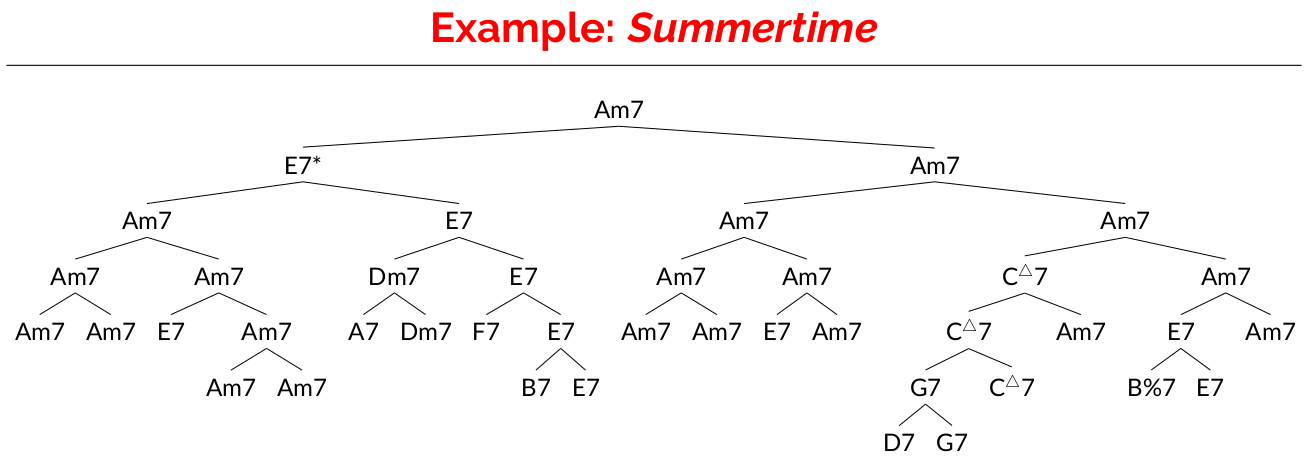
\includegraphics[height=60mm, width=125mm]{z_images/2_etat_de_l_art/summertime_tree.png}
\end{figure}

\cite{rohrmeier2020towards} cherchent à caractériser la structure interne récursive des rythmes musicaux en utilisant une grammaire formelle.
Cela va au-delà du GTTM (?), qui ne propose pas de modèle du rythme, et soutient en outre que l'inférence de la structure rythmique hiérarchique profonde est centrale à la cognition musicale. En raison de la représentation conjointe de la structure rythmique et métrique dans le modèle, un analyseur syntaxique de la grammaire abstraite du rythme musical proposée instancie l'interprétation rythmique et l'inférence métrique en même temps.
\section*{Conclusion}
La plupart des travaux déjà entrepris se concentrent sur des méthodes de calcul pour la détection d'événements sonores de batterie à partir de signaux acoustiques ou sur la séparation entre les évènement sonore de batterie avec ceux des autres instruments dans un orchestre ou un groupe de musique \cite{2802}, ainsi que sur l'extraction de caractéristiques de bas niveau telles que la classe d'instrument et le moment de l'apparition du son. Très peu d'entre eux ont abordé la tâche de générer des partitions de batterie.
Nous avons décidé de compléter le travail qui concerne la batterie en commençant par l’endroit le moins pratiqué, à savoir la transcription du MIDI vers la partition.